\section{CQ1}
\subsubsection{Question}
How many different Confirmable PUT requests obtained an unsuccessful response from the local CoAP server?

\subsubsection{Answer}
The number of Confirmable PUT request that obtained an unsuccessful response from the local CoAP server is 22.

\subsubsection{Explanation}
We filter the Confirmable PUT requests to a local CoAP server with a filter: Confirmable requests have type 0, PUT requests have code 3.
\begin{verbatim}
coap && coap.type == 0 && coap.code == 3 && ip.src == ip.dst
\end{verbatim}
We get 26 filtered messages.

We filter the unsuccessful responses from a local CoAP server based on the code, which needs to be bigger or equal than 128.
\begin{verbatim}
coap && (coap.code >= 128) && ip.src == ip.dst
\end{verbatim}
We get 141 filtered messages.\\
In order to answer QC1, we should follow the UDP stream for all 26 requests and check the code associated to the response, checking that all requests are different, i.e. have different token.\\
To avoid doing this manually, we used a Python script written using PyShark library.

\begin{python}
import pyshark
import sys
import re
def answer_cq1(capture):
    requests = {}
    responses = {}
    for pkt in capture:
        try:
            # check local server 
            if 'IP' not in pkt or pkt.ip.src != pkt.ip.dst:
                continue
            # check CoAP layer
            if 'COAP' in pkt:
                coap = pkt.coap
                # get fields 
                coap_type = int(coap.get_field('type')) if hasattr(coap, 'type') else None
                coap_code = int(coap.get_field('code')) if hasattr(coap, 'code') else None
                token = coap.get_field('token') if hasattr(coap, 'token') else None
                if coap_type is None or coap_code is None or token is None:
                    continue
                if coap_type == 0 and coap_code == 3:
                    # Confirmable PUT request 
                    requests[token] = pkt
                elif coap_code >= 128:
                    # unsuccessful response  
                    responses[token] = pkt
        except Exception:
            continue
    count = sum(1 for token in requests if token in responses)
    return count
def main():
    if len(sys.argv) != 2:
        print("pcap file not provided")
        sys.exit(1)
    pcap_file = sys.argv[1]
    capture = pyshark.FileCapture(pcap_file, keep_packets=False)    
    print(answer_cq1(capture))
    capture.close()
if __name__ == "__main__":
    main()
\end{python}

Running this script, we get a result of 22 requests.

\section{CQ2}
\subsubsection{Question}
How many CoAP resources in the coap.me public server received the same number of unique Confirmable and Non Confirmable GET requests?\\
Assuming a resource receives X different CONFIRMABLE requests and Y different NONCONFIRMABLE GET requests, how many resources have X=Y, with X>0?

\subsubsection{Answer}
The number of CoAP resources in the coap.me public server that received the same number of unique Confirmable and Non Confirmable GET requests is 3.

\subsubsection{Explanation}
We can find the IP address of coap.me server with a Wireshark filter.
\begin{verbatim}
dns.qry.name == "coap.me"
\end{verbatim}
We can see that the IP is 134.102.218.18.\\

We can find the Confirmable GET requests issued to coap.me with the following filter:
\begin{verbatim}
coap.type == 0 && coap.code == 1 && ip.dst==134.102.218.18
\end{verbatim}
While Non Confirmable GET requests to coap.me can be found with this filter:
\begin{verbatim}
coap.type == 1 && coap.code == 1 && ip.dst==134.102.218.18
\end{verbatim}
We find 39 Confirmable request and 31 Non Confirmable ones and we would need to count the number of requests for each resource.\\
Instead, we can use a PyShark algorithm to do the same.
\begin{python}
import pyshark
import re
import sys

def answer_cq2(capture):
    # IP found with Wireshark filter
    coap_me_ip = "134.102.218.18"
    resource_stats = {}
    # find target requests and responses
    for pkt in capture:
        try:
            # check destination is coap.me
            if 'IP' not in pkt or pkt.ip.dst != coap_me_ip:
                continue
            # check CoAP layer
            if 'COAP' in pkt:
                coap = pkt.coap
                # get fields 
                coap_type = int(coap.get_field('type')) if hasattr(coap, 'type') else None
                coap_code = int(coap.get_field('code')) if hasattr(coap, 'code') else None
                token = coap.get_field('token') if hasattr(coap, 'token') else None
                resource = coap.get_field('opt_uri_path') if hasattr(coap, 'opt_uri_path') else None                
                if coap_type is None or coap_code is None or token is None or resource is None:
                    continue
                # check GET request 
                if coap_code != 1:
                    continue
                if resource not in resource_stats:
                    resource_stats[resource] = {'conf': set(), 'nonconf': set()}
                if coap_type == 0:
                    # Confirmable
                    resource_stats[resource]['conf'].add(token)
                elif coap_type == 1:
                    # Non Confirmable
                    resource_stats[resource]['nonconf'].add(token)
        except Exception:
            continue
    # count target resources 
    count = 0
    for stats in resource_stats.values():
        if len(stats['conf']) == len(stats['nonconf']) and len(stats['conf']) > 0:
            count += 1
    return count

def main():
    if len(sys.argv) != 2:
        print("pcap file not provided")
        sys.exit(1)
    pcap_file = sys.argv[1]
    capture = pyshark.FileCapture(pcap_file, keep_packets=False)
    print(answer_cq2(capture))
    capture.close()

if __name__ == "__main__":
    main()
\end{python}

Running the algorithm, we find out that 3 resources have the same number of Confirmable and Non Confirmable GET requests.

\section{CQ3}
\subsubsection{Question}
How many different MQTT clients subscribe to the public broker HiveMQ using multi-level wildcards?

\subsubsection{Answer}
The number of clients who subscribe to the public broker HiveMQ using multi-level wildcards is 4.

\subsubsection{Explanation}
In order to find the IP address of the HiveMQ broker, we filter the response of the DNS server using the following Wireshark filter:
\begin{verbatim}
dns.qry.name == "broker.hivemq.com"
\end{verbatim}
All DNS responses return 3 addresses: 18.192.151.104, 35.158.34.213 and 35.158.43.69.

We use a second filter to find SUBSCRIBE messages, with message type 8, sent to HiveMQ broker, to one of the IP addresses found above, with a multi-level wildcard, ending with "\#": 
\begin{verbatim}
mqtt && mqtt.msgtype == 8 && 
(ip.dst == 18.192.151.104 || ip.dst == 35.158.34.213 
|| ip.dst == 35.158.43.69) && mqtt.topic contains "#"
\end{verbatim}
We find out that HiveMQ broker receives 6 messages of this type, all at the IP address 18.192.151.104.

\begin{figure}[H]
    \centering
    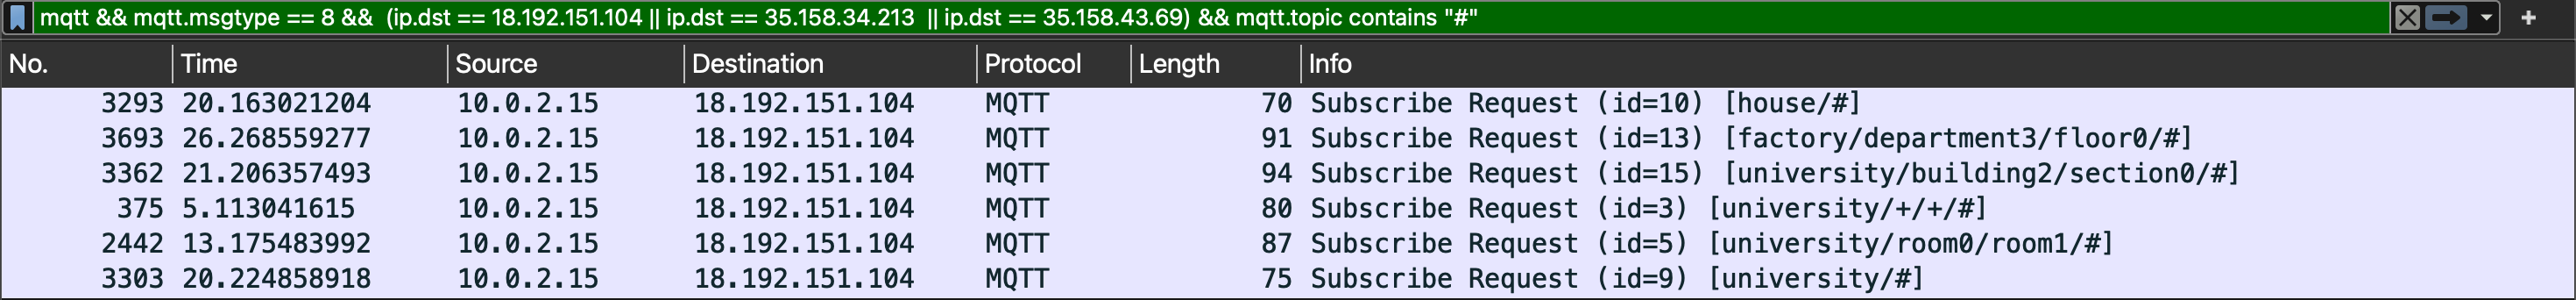
\includegraphics[width=\linewidth, height=0.85\textheight, keepaspectratio]{QC3_1.png}
    \caption{SUBSCRIBE messages to HiveMQ broker with "\#"}
\end{figure}

Since the question asks for the number of MQTT clients who subscribe, we need to identify the clients who sent these messages. For each message, we select the TCP stream, which identifies the client.\\

\begin{table}[H]
\centering 
\begin{tabular}{| c | c |}
	\hline 
	\rowcolor{bluepoli!40}
	\textbf{Message number} & \textbf{TCP stream}\T\B \\
	\hline 
	375 & 8 \T\B\\
	2442 & 15 \T\B\\
	3293 & 20 \T\B\\
	3303 & 15 \T\B\\
	3362 & 3 \T\B\\
	3693  & 15 \T\B\\
	\hline
\end{tabular}
\\[10pt]
\caption{TCP streams}
\label{table:tcp_streams}
\end{table}

Since there are 4 TCP streams, the 6 messages have been sent by 4 different client.	\\
We can also find the Client ID of these clients by finding the CONNECT message, of type 1, they sent to the broker. For the TCP stream 8, we can use the following filter:
\begin{verbatim}
mqtt && mqtt.msgtype == 1 && tcp.stream == 8
\end{verbatim}
The same filter with different TCP stream can be used for other clients.

\begin{table}[H]
\centering 
\begin{tabular}{| c | c |}
	\hline 
	\rowcolor{bluepoli!40}
	\textbf{TCP stream} & \textbf{Client ID}\T\B \\
	\hline 
	3 & cpoepjzkhibxgjiu \T\B\\
	8 & dzcxnwdqef \T\B\\
	15 & tukvxesuhe \T\B\\
	20 & fcthvjikxjul \T\B\\
	\hline
\end{tabular}
\\[10pt]
\caption{Client IDs table}
\label{table:client_ids_table}
\end{table}

\section{CQ4}
\subsubsection{Question}
How many different MQTT clients specify a Last Will Message to be directed to a topic having as first level "university"?

\subsubsection{Answer}
The number of clients who specify a Last Will Message to be directed to a topic having as first level "university" is 1.

\subsubsection{Explanation}
MQTT clients can specify a Last Will Message in the CONNECT message. In order to find the described messages, we filter CONNECT messages, of type 1, with a Last Will Topic:
\begin{verbatim}
mqtt && mqtt.msgtype == 1 && mqtt.willtopic
\end{verbatim}
We find four messages, but only one of them has a Last Will Topic having as first level "university".\\

\begin{figure}[H]
    \centering
    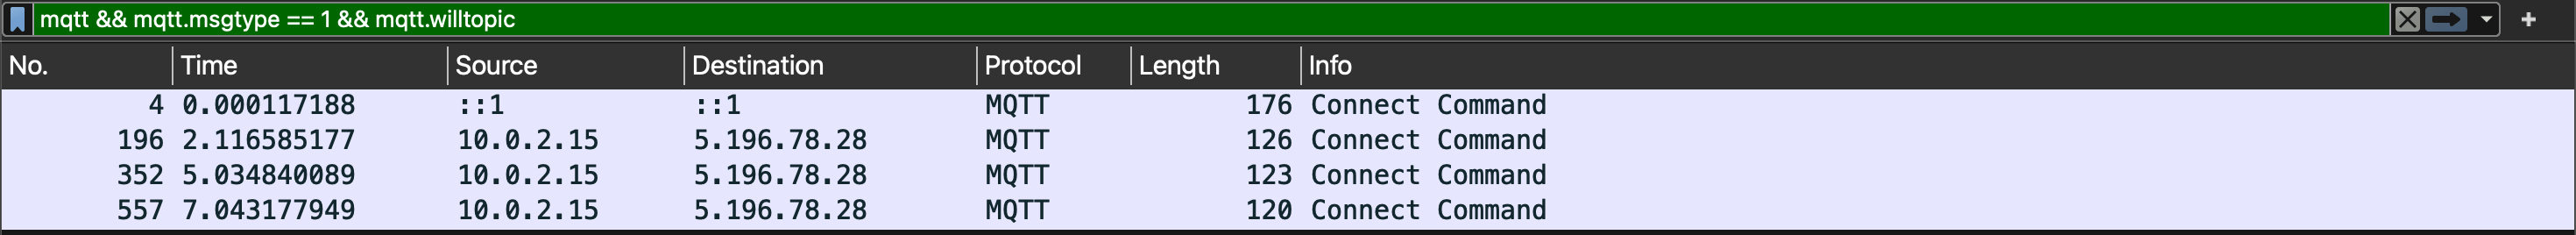
\includegraphics[width=\linewidth, height=0.85\textheight, keepaspectratio]{QC4_1.png}
    \caption{CONNECT messages specifying a Last Will Topic}
\end{figure}

We can find the result by enriching the filter and avoiding manually checking the topics, using the following filter:
\begin{verbatim}
mqtt && mqtt.msgtype == 1 && mqtt.willtopic matches "^university"
\end{verbatim}
Using this filter, we directly get the only message asked by CQ4.

\begin{figure}[H]
    \centering
    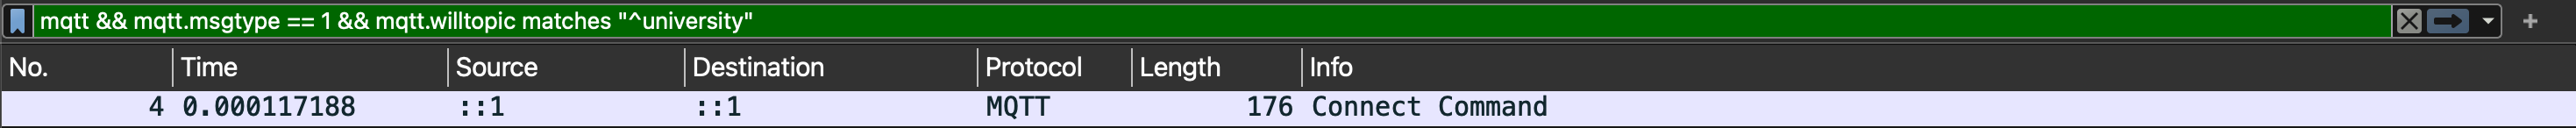
\includegraphics[width=\linewidth, height=0.85\textheight, keepaspectratio]{QC4_2.png}
    \caption{CONNECT messages specifying a Last Will Topic starting with "university"}
\end{figure}

\section{CQ5}
\subsubsection{Question}
How many MQTT subscribers receive a last will message derived from a subscription without a wildcard?

\subsubsection{Answer}
The number of subscribers who receive a Last Will Message derived from a subscription without a wildcard is 3.

\subsubsection{Explanation}
We start by identifying the possible Last Will Messages (LWM). To do so, we find all the CONNECT messages, with message type 1, that specify a LWM.
\begin{verbatim}
mqtt && mqtt.msgtype== 1 && mqtt.willmsg
\end{verbatim}

We find four messages.
\begin{figure}[H]
    \centering
    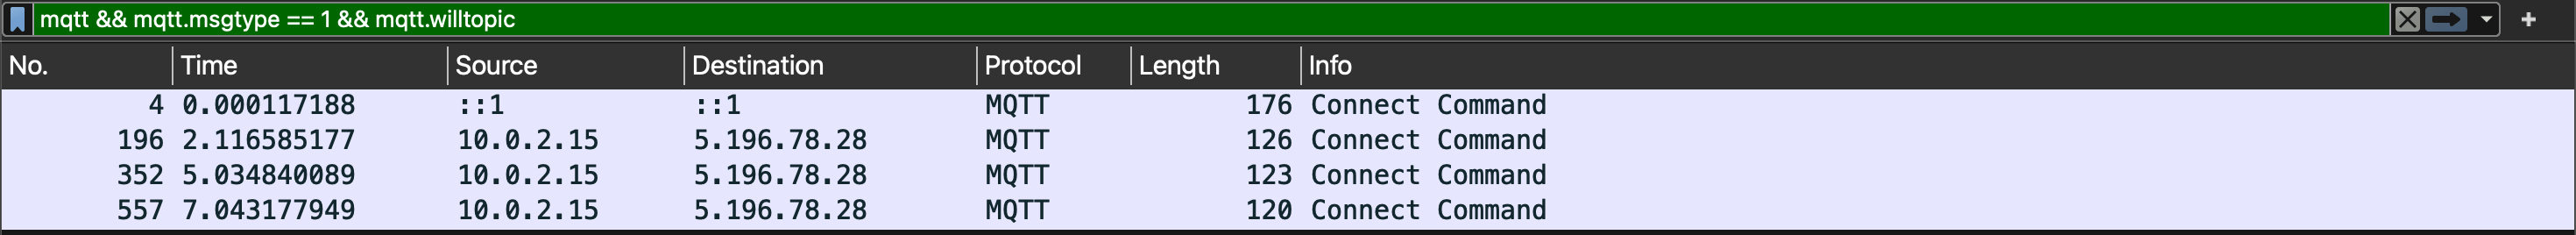
\includegraphics[width=\linewidth, height=0.85\textheight, keepaspectratio]{QC5_1.png}
    \caption{CONNECT messages specifying a LWM}
\end{figure}

These messages specify the Last Will Messages, which we don't report in the table, and Last Will Topics.
\begin{table}[H]
\centering 
\begin{tabular}{| c | c | c |}
	\hline 
	\rowcolor{bluepoli!40}
	\textbf{Message number} & \textbf{Destination} & \textbf{Last Will Topic}\T\B \\
	\hline 
	4 & ::1 & university/department12/room1/temperature \T\B\\
	196 & 5.196.78.28 & metaverse/room2/floor4 \T\B\\
	352 & 5.196.78.28 & hospital/facility3/area3 \T\B\\
	557 & 5.196.78.28 & metaverse/room2/room2 \T\B\\
	\hline
\end{tabular}
\\[10pt]
\caption{Last Will Topics}
\end{table}

Starting from the first Last Will Topic (LWT), we filter all PUBLISH messages with that topic and with same message as the LWM, found in the CONNECT message.
\begin{verbatim}
mqtt && mqtt.msgtype==3 && 
mqtt.topic == "university/department12/room1/temperature" && 
mqtt.msg contains 6572726f723a20612056495020436c69656e74206a7573742064696564
\end{verbatim}

We find four messages:
\begin{figure}[H]
    \centering
    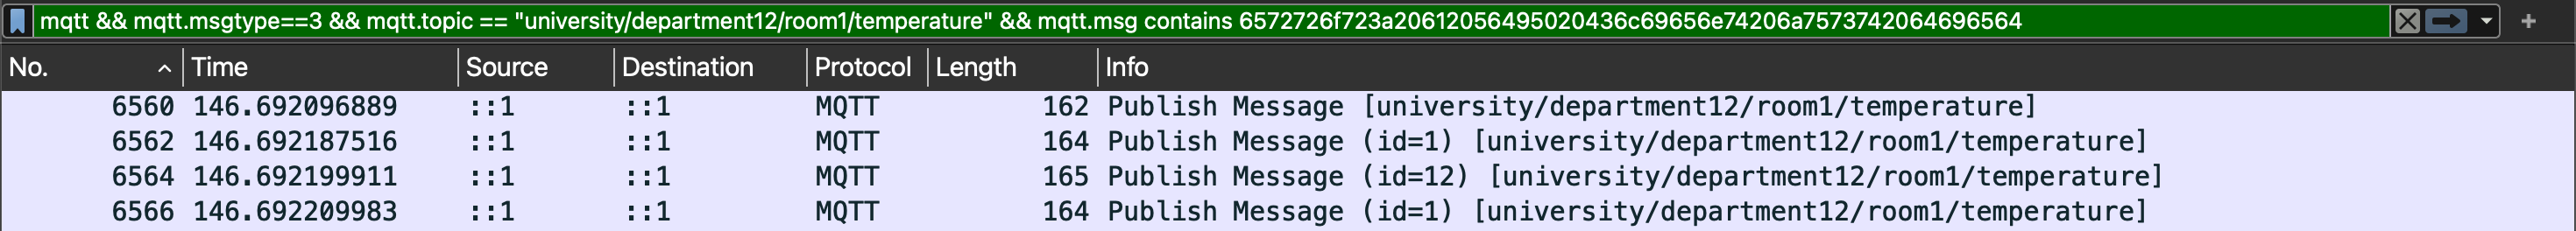
\includegraphics[width=\linewidth, height=0.85\textheight, keepaspectratio]{QC5_2.png}
    \caption{LWM with topic "university/department12/room1/temperature"}
\end{figure}

By looking at the messages, we can see a TCP Reset message, representing an hard disconnection, followed by four Last Will Messages sent by the broker, on port 1883, to different client, on different ports and using different TCP streams.
\begin{figure}[H]
    \centering
    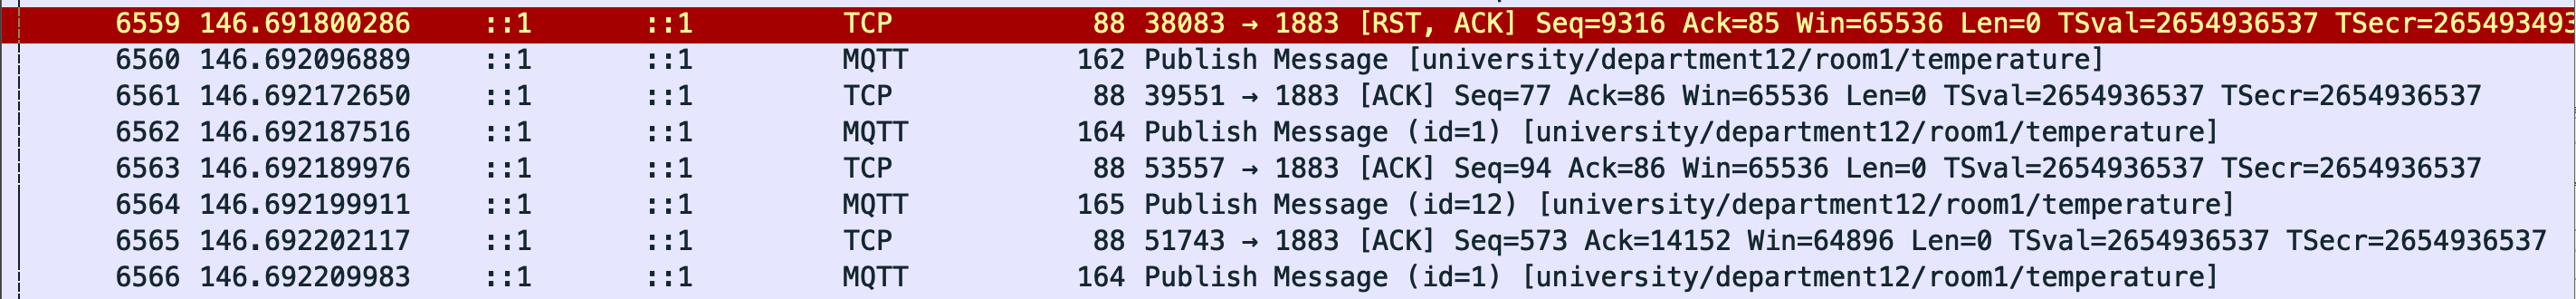
\includegraphics[width=\linewidth, height=0.85\textheight, keepaspectratio]{QC5_3.png}
    \caption{TCP Reset and Last Will Messages}
\end{figure}

The clients who receive the LWM are grouped in the following table.
\begin{table}[H]
\centering 
\begin{tabular}{| c | c | c |}
	\hline 
	\rowcolor{bluepoli!40}
	\textbf{Message number} & \textbf{Subscriber port} & \textbf{TCP stream}\T\B \\
	\hline 
	6560 & 39551 & 2 \T\B\\
	6562 & 53557 & 6 \T\B\\
	6564 & 51743 & 10 \T\B\\
	6566 & 41789 & 14 \T\B\\
	\hline
\end{tabular}
\\[10pt]
\caption{Last Will Topics}
\end{table}

In order to answer to QC5, we need to find which of these clients subscribed to the Last Will Topic without a wildcard. We can do so by filtering the SUBSCRIBE messages, with message type 8, with the correct TCP stream. For each of them we also find the CONNECT message and Client ID.
\begin{verbatim}
mqtt && mqtt.msgtype == 8 && mqtt.topic matches "^university" && 
(tcp.stream == 2 || tcp.stream == 6 || tcp.stream == 10 || tcp.stream == 14)
\end{verbatim}

\begin{figure}[H]
    \centering
    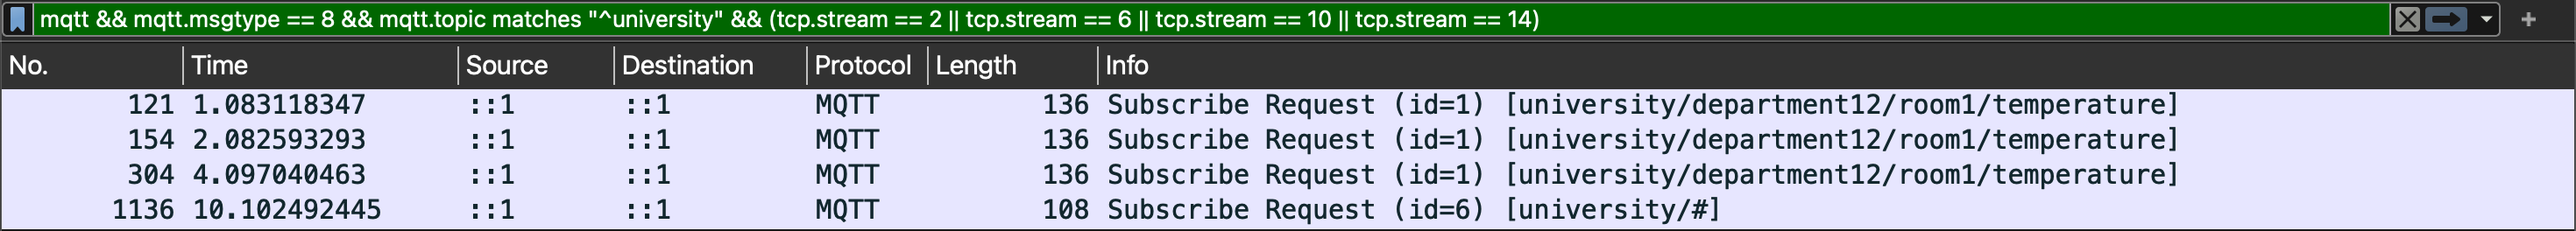
\includegraphics[width=\linewidth, height=0.85\textheight, keepaspectratio]{QC5_4.png}
    \caption{TCP Reset and Last Will Messages}
\end{figure}

We can see that only three out of four clients subscribed to the Last Will Topic without a wildcard.

\begin{table}[H]
\centering 
\begin{tabular}{| c | c | c |}
	\hline 
	\rowcolor{bluepoli!40}
	\textbf{TCP stream} & \textbf{Client ID} & \textbf{Specified topic}\T\B \\
	\hline 
	2 & auyvhrhdudnm & university/department12/room1/temperature \T\B\\
	6 & ntpiopsqc & university/department12/room1/temperature \T\B\\
	10 & zmjnxudohrkaegmh & university/\# \T\B\\
	14 & mjdocmjxt & university/department12/room1/temperature \T\B\\
	\hline
\end{tabular}
\\[10pt]
\caption{Specified topics}
\end{table}

For what concerns the other three Last Will Topics, we filter all PUBLISH messages, with message type 3, from the broker, with IP 5.196.78.28.
\begin{verbatim}
mqtt && ip.src == 5.196.78.28 && mqtt.msgtype == 3 
\end{verbatim}
We don't find any result, which means that the broker doesn't publish any message, nor LWM.\\
We conclude that three clients receive a LWM from a subscription without a wildcard, all of them from the first topic.

\section{CQ6}
\subsubsection{Question}
How many MQTT publish messages directed to the public broker mosquitto are sent with the retain option and use QoS “At most once”?

\subsubsection{Answer}
The number of publish messages directed to the public broker mosquitto are sent with the retain option and use QoS “At most once” is 208.

\subsubsection{Explanation}
In order to find the IP address of the public broker mosquitto, we filter the response of the DNS server using the following Wireshark filter:
\begin{verbatim}
dns.qry.name == "test.mosquitto.org"
\end{verbatim}
Al DNS responses return the same IP address: 5.196.78.28.\\
Now we need a second filter in order to obtain all the publish messages that satisfy the question:
\begin{verbatim}
mqtt.msgtype == 3 and mqtt.qos == 0 and mqtt.retain == 1 and ip.dst == 5.196.78.28
\end{verbatim}
We find 208 results, so we can conclude that the number of packets that satisfy all the constraints is 208.

\section{CQ7}
\subsubsection{Question}
How many MQTT-SN messages on port 1885 are sent by the clients to a broker in the local machine?

\subsubsection{Answer}
The number of MQTT-SN messages on port 1885 sent by the clients to a broker in the local machine is 0.

\subsubsection{Explanation}
Natively MQTT-SN is not recognised by Wireshark and therefore a preliminary operation is required. By going into the settings we can set 1885 as the port of MQTT-SN.
Since MQTT-SN is a udp protocol, in order to filter all the messages using MQTT-SN we can use this Wireshark filter
\begin{verbatim}
udp.dstport == 1885
\end{verbatim}
\begin{figure}[H]
    \centering
    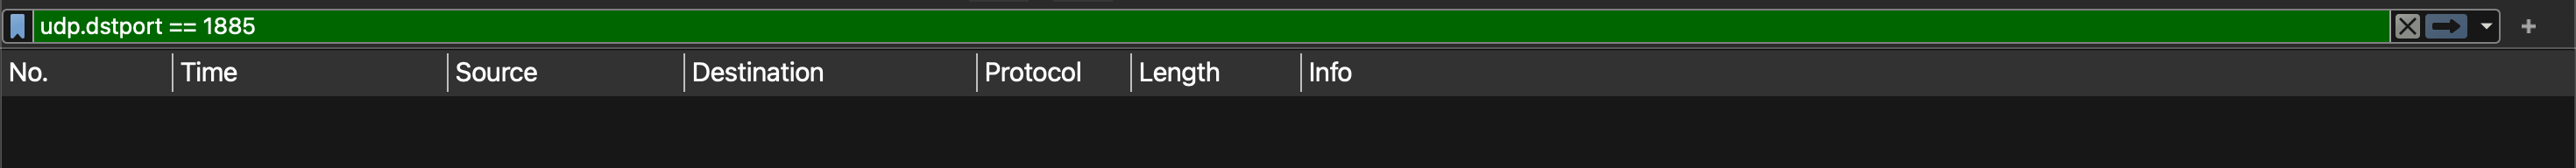
\includegraphics[width=\linewidth, height=0.85\textheight, keepaspectratio]{QC7_1.png}
    \caption{Udp destination port 1885}
\end{figure}
\begin{figure}[H]
    \centering
    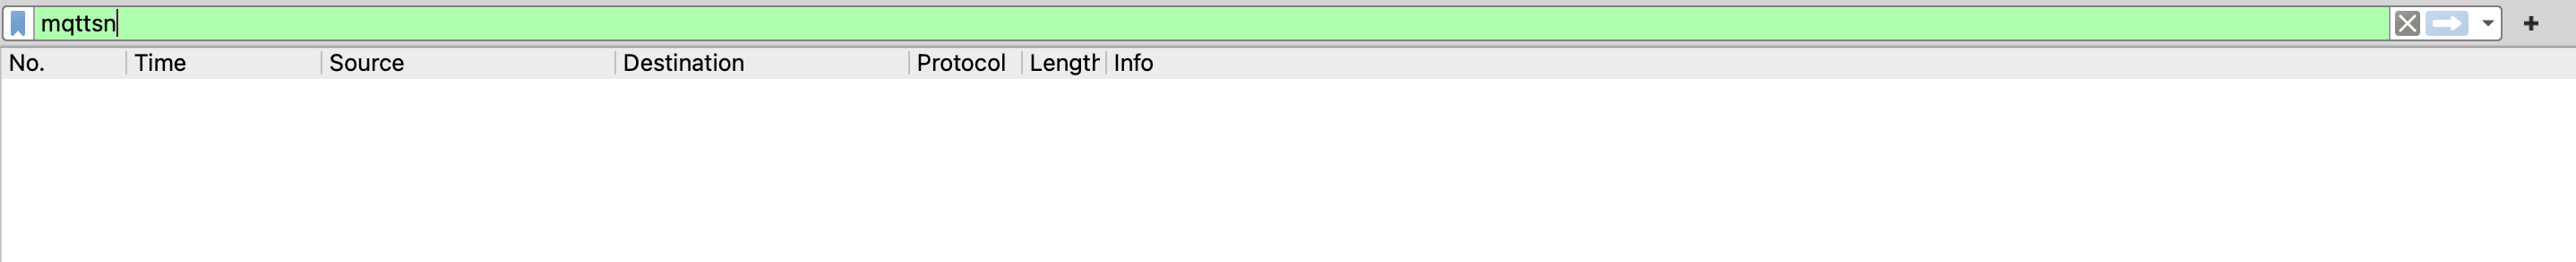
\includegraphics[width=\linewidth, height=0.85\textheight, keepaspectratio]{QC7_2.png}
    \caption{MQTT-SN messages}
\end{figure}
However, both this filter and the standard ‘mqttsn’ filter do not return a single packet, so to be sure that the result is 0, it is possible to carry out a further check knowing that MQTT-SN always has topic length equal to 2:
\begin{verbatim}
mqtt.topic_len == 2
\end{verbatim}
\begin{figure}[H]
    \centering
    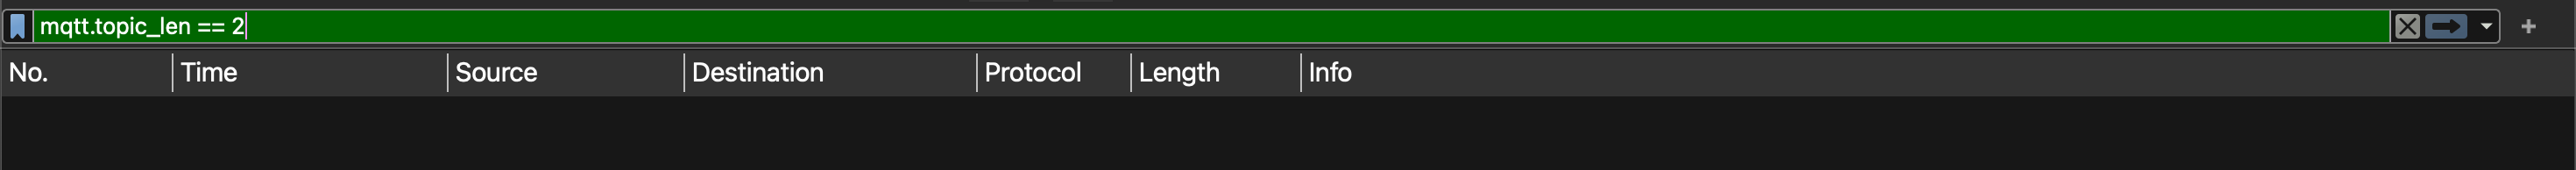
\includegraphics[width=\linewidth, height=0.85\textheight, keepaspectratio]{QC7_3.png}
    \caption{MQTT messages with topic length 2}
\end{figure}
But this filter also gives no results, so we can conclude that there are no MQTT-SN messages sent on port 1885 by the clients to a broker in the local machine.

\section{References}
In this section we provide a set of references we used.
\begin{itemize}
	\item \url{https://datatracker.ietf.org/doc/html/rfc7641}
	\item \url{https://docs.oasis-open.org/mqtt/mqtt/v5.0/os/mqtt-v5.0-os.html}
\end{itemize}
























